\section{随机目标与梯度估计}
\label{sec:sgd-objectives}

只读部分信息时，手里得到的向量和当前点的真梯度是什么关系？回答它需要先说清要最小化的是哪个目标，再说清“随机”来自哪里，最后给出“这个读数可以当作梯度用”的准确含义。读取的顺序也会改变这一含义，放在本节最后讨论。

\subsection{有限和目标}
\label{sec:sgd-finite-sum}

先看最常见的情形：数据已经固定，目标是$N$项的平均。

\paragraph{目标与完整梯度}
设$f_i:\mathbb{R}^n\to\mathbb{R}$，$i=1,\ldots,N$，都可微。\term{有限和目标}（finite-sum objective）是
\begin{equation}
 f(\bm{x})=\frac{1}{N}\sum_{i=1}^{N}f_i(\bm{x}).
 \label{eq:sgd-finite-sum}
\end{equation}
求导对有限和可以逐项进行，所以完整梯度是各项梯度的平均：
\begin{equation}
 \nabla f(\bm{x})=\frac{1}{N}\sum_{i=1}^{N}\nabla f_i(\bm{x}).
 \label{eq:sgd-full-gradient}
\end{equation}
要得到它，必须把$N$项都计算一遍。本章把计算一项梯度称为一次\emph{读取}，完整梯度的代价是$N$次读取。

\paragraph{均匀抽取一项}
现在换一种获取信息的方式：在$\{1,\ldots,N\}$中均匀抽一个下标$i$，只计算$\nabla f_i(\bm{x})$。每个下标的概率都是$1/N$，因此对这次抽样求平均，得到
\begin{equation}
 \mathbb{E}_i[\nabla f_i(\bm{x})]=\sum_{i=1}^{N}\frac{1}{N}\nabla f_i(\bm{x})=\nabla f(\bm{x}).
 \label{eq:sgd-uniform-mean}
\end{equation}
目标函数并没有变，变的只是当前拿到的信息：从全部$N$项变成其中一项。

这就像估计全校的平均身高：不必量遍每个人，随机问一个人，他的身高在平均意义上就是全校的平均。学生对应目标项，身高对应该项的梯度，全校平均对应完整梯度。这个类比有两处失效。身高不随时间改变，而$\nabla f_i(\bm{x})$随$\bm{x}$改变，每走一步都要重新估计。另外，估计身高只要结果，估计梯度还要照着它走路，走错的后果会带到下一步。

\paragraph{贯穿全章的三项目标}
取一元、三项的目标，每项是一条抛物线：
\begin{equation}
 f_i(x)=\frac{a_i}{2}(x-b_i)^2,\qquad
 (a_1,a_2,a_3)=(1,2,3),\qquad
 (b_1,b_2,b_3)=(-3,0,3).
 \label{eq:sgd-example-terms}
\end{equation}
三项写出来是
\[
 f_1(x)=\frac12(x+3)^2,\qquad f_2(x)=x^2,\qquad f_3(x)=\frac32(x-3)^2.
\]

把三项相加再除以$3$。二次项系数是$\tfrac16+\tfrac13+\tfrac12=1$，一次项系数是$1+0-3=-2$，常数项是$\tfrac32+0+\tfrac92=6$，所以
\begin{equation}
 f(x)=x^2-2x+6=(x-1)^2+5.
 \label{eq:sgd-example-objective}
\end{equation}
于是最小点和最优值是
\[
 x^\star=1,\qquad f^\star=5.
\]

各项的梯度$f_i'(x)=a_i(x-b_i)$与完整梯度是
\begin{equation}
 f_1'(x)=x+3,\qquad f_2'(x)=2x,\qquad f_3'(x)=3x-9,\qquad f'(x)=2x-2.
 \label{eq:sgd-example-gradients}
\end{equation}
这里$f$的曲率是$2$，所以$L=\mu=2$；各项自身的曲率是$L_i=a_i$，最大为$3$。

在$x=2$处，三项的读数和完整梯度是
\[
 f_1'(2)=5,\qquad f_2'(2)=4,\qquad f_3'(2)=-3,\qquad f'(2)=2.
\]
第三项的读数是负的，说明它主张向右走，而完整梯度要求向左走。最优点$x^\star=1$恰在左边，听第三项的话就走反了。在最优点，三项读数为$(4,2,-6)$，它们的和是零，但没有一项是零。完整梯度已经停下，单项读数并没有停下。这两个现象会贯穿全章。

\begin{BookInlineFigure}
  \centering
  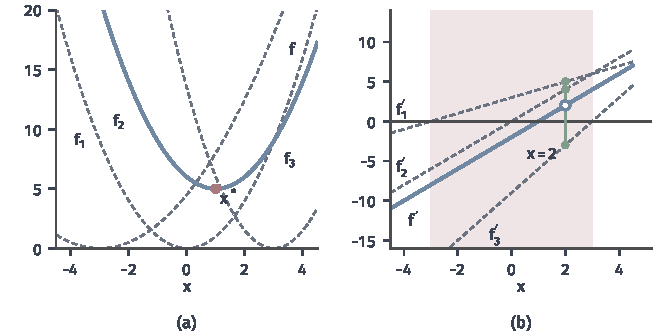
\includegraphics[width=112mm]{figures/05-optimization/05-stochastic-optimization/matplotlib/sgd-term-gradients/figure.pdf}
  \caption{三项目标~\eqref{eq:sgd-example-terms}。(a)虚线是三条单项抛物线$f_1,f_2,f_3$，实线是它们的平均$f$，红点是$f$的最小点$x^\star=1$，各项的最小点都不在这里。(b)虚线是单项导数，实线是$f'$。红底区间$[-3,3]$内三项导数不同号；区间外三项同号，都指向区间。竖线段标出$x=2$处的三个读数$5,4,-3$，空心点是它们的平均$2$。}
  \label{fig:sgd-term-gradients}
\end{BookInlineFigure}

图~\ref{fig:sgd-term-gradients}(b)给出了分歧发生的位置。三条单项导数的零点是$-3,0,3$，在这三个数之外，三项一致地指向同一边，读哪一项方向都对。进入$[-3,3]$后各项开始争执。所以离解还远时，单项读数和完整梯度方向相同；离解越近，分歧越明显。

\paragraph{归一化、正则项与读取成本}
式~\eqref{eq:sgd-finite-sum}里的$1/N$不是可有可无的约定。若目标写成不除以$N$的总和，最小点不变，但梯度和光滑常数都放大$N$倍，同一个数值的步长含义完全不同。本章一律使用平均的写法，步长$\alpha$可以脱离$N$来讨论。

许多目标还带确定的正则项$r$，例如$r(\bm{x})=\tfrac{\gamma}{2}\lVert\bm{x}\rVert_2^2$：
\begin{equation}
 f(\bm{x})=\frac{1}{N}\sum_{i=1}^{N}f_i(\bm{x})+r(\bm{x}).
 \label{eq:sgd-finite-sum-regularized}
\end{equation}
$r$不依赖数据项，它的梯度每步都能精确算出，无需抽样。读数应写成$\nabla f_i(\bm{x})+\nabla r(\bm{x})$。如果把$r$放进每一项，写成$f_i+r$，结果相同；要避免的是只在抽到某些项时才加入$r$，或把系数随$N$改变而不作说明。

计数时要分清两种成本：一次读取是对单项的梯度计算，一次更新是对$\bm{x}$的修改。完整梯度下降每次更新$N$次读取，只读一项时每次更新一次读取。比较算法时，本章以读取次数为主要的计量单位。

\subsection{期望目标}
\label{sec:sgd-expected}

很多问题中项数不是固定的$N$。观测可以源源不断地取得，或者目标本来就是在某个分布上的平均。

\paragraph{从有限平均到期望}
设$\bm{\xi}$是可以抽样的随机变量，对每个$\bm{\xi}$的取值有函数$\phi(\bm{x};\bm{\xi})$。\term{期望目标}（expected objective）是
\begin{equation}
 f(\bm{x})=\mathbb{E}_{\bm{\xi}}[\phi(\bm{x};\bm{\xi})].
 \label{eq:sgd-expected-objective}
\end{equation}
有限和是特例：取$\bm{\xi}$为均匀分布的下标$i$，$\phi(\bm{x};i)=f_i(\bm{x})$。三项目标正是这样，$f$是三点分布上的期望。

一般情况下无法把所有取值列出来，也无法求出$f$，却能抽样。这样就有两种不同的做法。

一种是\emph{直接优化期望}：每一步抽一个新样本，把它的梯度用于更新。每个样本只用一次，读取总数等于样本总数，要最小化的始终是式~\eqref{eq:sgd-expected-objective}。另一种是\emph{先固定一批样本}：一次抽定$\bm{\xi}_1,\ldots,\bm{\xi}_N$，得到
\[
 f_N(\bm{x})=\frac{1}{N}\sum_{i=1}^{N}\phi(\bm{x};\bm{\xi}_i),
\]
然后把$f_N$当作有限和目标反复读取。这时算法解的是$f_N$，它的解一般不是$f$的解。

\begin{BookInlineFigure}
  \centering
  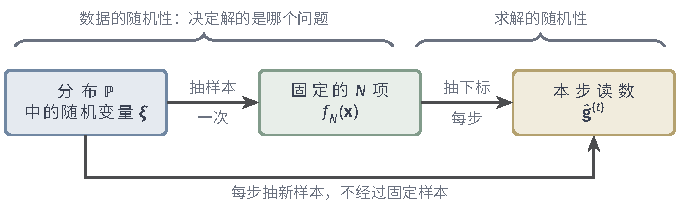
\includegraphics[width=112mm]{figures/05-optimization/05-stochastic-optimization/tikz/sgd-two-randomness/figure.pdf}
  \caption{两层随机性。上方路线先抽定$N$个样本，得到确定的有限和$f_N$，之后每步只对下标抽样。下方路线不经过固定样本，每步直接抽新样本。第一层随机性决定了算法解的是哪个问题，第二层只影响算法解这个问题的过程。}
  \label{fig:sgd-two-randomness}
\end{BookInlineFigure}

图~\ref{fig:sgd-two-randomness}区分了这两层随机性。举一个具体的例子：取$\phi(x;\xi)=\tfrac12(x-\xi)^2$，$\xi$的均值为$1$。期望目标的最小点是$1$，而$f_N$的最小点是样本均值$\bar{\xi}_N$，它随样本变化。无论优化做得多准，都只能精确得到$\bar{\xi}_N$；$\bar{\xi}_N$与$1$的差属于数据造成的统计误差。本章固定目标，只研究优化误差。统计误差的大小可参考\BookChapterRef{chap:finite-sample-error-bounds}{卷八第4章“有限样本的误差上界”}。

\paragraph{逐样本求导的条件}
随机梯度要求$\nabla\phi(\bm{x};\bm{\xi})$的期望等于$\nabla f(\bm{x})$，也就是导数和期望可以交换。有限和中这一步只是有限项相加，期望的情形需要条件。

\begin{lemma}[逐样本求导]
\label{lem:sgd-differentiate-expectation}
设$\bm{x}$有开球邻域$\bm{U}$，$\phi(\bm{x};\bm{\xi})$可积。若几乎所有$\bm{\xi}$使$\phi(\cdot;\bm{\xi})$在$\bm{U}$上可微，且存在可积函数$M(\bm{\xi})$，使
\begin{equation}
 \lVert\nabla\phi(\bm{y};\bm{\xi})\rVert_2\leq M(\bm{\xi}),\qquad \bm{y}\in\bm{U},
 \label{eq:sgd-local-domination}
\end{equation}
则$f$在$\bm{x}$处可微，并且
\begin{equation}
 \nabla f(\bm{x})=\mathbb{E}_{\bm{\xi}}[\nabla\phi(\bm{x};\bm{\xi})].
 \label{eq:sgd-gradient-expectation}
\end{equation}
\end{lemma}

\begin{proof}
记$\bm{v}(\bm{\xi})=\nabla\phi(\bm{x};\bm{\xi})$。由式~\eqref{eq:sgd-local-domination}，$\bm{v}$可积。取$\bm{h}^{(k)}\to\bm{0}$，$\bm{h}^{(k)}\neq\bm{0}$，且$\bm{x}+\bm{h}^{(k)}\in\bm{U}$，令
\[
 R_k(\bm{\xi})=\frac{\phi(\bm{x}+\bm{h}^{(k)};\bm{\xi})-\phi(\bm{x};\bm{\xi})-\langle\bm{v}(\bm{\xi}),\bm{h}^{(k)}\rangle}{\lVert\bm{h}^{(k)}\rVert_2}.
\]

对几乎所有$\bm{\xi}$，由可微性有$R_k(\bm{\xi})\to0$。沿线段使用中值定理，并由式~\eqref{eq:sgd-local-domination}，得到
\[
 \lvert R_k(\bm{\xi})\rvert\leq2M(\bm{\xi}).
\]
这说明$\phi(\bm{x}+\bm{h}^{(k)};\cdot)$也可积，$f$在这些点有定义。

控制收敛定理给出$\mathbb{E}[R_k]\to0$，定理的条件和证明见\BookChapterRef{chap:integration}{卷四第6章“积分”}。序列$\bm{h}^{(k)}$是任取的，所以这正是$f$在$\bm{x}$处以$\mathbb{E}[\bm{v}]$为梯度可微的定义。
\end{proof}

条件~\eqref{eq:sgd-local-domination}去掉后结论可以错得很彻底。取$\xi$在$(0,1)$上均匀，$\phi(x;\xi)$是示性函数：当$\xi\leq x$时取$1$，否则取$0$。对$x\in(0,1)$，期望目标是$f(x)=x$，导数处处为$1$。但对每个固定的$\xi$，除$x=\xi$这一点外函数都是常数，逐样本导数是$0$，平均之后还是$0$。跳跃点带来的贡献被逐样本求导完全漏掉了。对照引理的条件，落在$\bm{U}$内的$\xi$使$\phi(\cdot;\xi)$在$y=\xi$处不连续，“在整个邻域上可微”这一条不成立；只在$x$这一点几乎处处可微是不够的。

分布本身依赖$\bm{x}$时，式~\eqref{eq:sgd-gradient-expectation}不能直接用，因为抽样分布也在变。常用的处理是把随机性移到不依赖$\bm{x}$的变量上（重参数化），或用分布密度的对数导数作权重（得分函数估计），可参考\BookChapterRef{chap:expectation-gradient-estimation}{卷七第33章“含参期望的梯度估计”}。本章下文只讨论分布不依赖$\bm{x}$的情形。

\subsection{条件无偏与读数误差}
\label{sec:sgd-unbiased}

式~\eqref{eq:sgd-uniform-mean}是对固定的$\bm{x}$写的。迭代中$\bm{x}^{(t)}$本身由前面的抽样决定，也是随机的。需要一个能处理“当前点已经随机地到了这里”的说法。

\paragraph{历史与条件期望}
把第$t$步抽样之前已经发生的一切称为\emph{历史}，记为$\mathcal{F}^{(t)}$：初始点、前$t$次抽到的下标。给定历史，$\bm{x}^{(t)}$就是一个确定的点。条件期望$\mathbb{E}[\cdot\mid\mathcal{F}^{(t)}]$可以这样理解：把过去冻结，只对第$t$步的新抽样求平均。

本章反复使用条件期望的两条规则。历史已知的量可以提到条件期望外面：
\begin{equation}
 \mathbb{E}[\,\bm{u}^\top\bm{v}\mid\mathcal{F}^{(t)}]=\bm{u}^\top\mathbb{E}[\bm{v}\mid\mathcal{F}^{(t)}],\qquad \bm{u}\text{由}\mathcal{F}^{(t)}\text{确定}.
 \label{eq:sgd-pull-out}
\end{equation}
先对新抽样平均、再对历史平均，等于直接取总平均，即全期望公式：
\begin{equation}
 \mathbb{E}\bigl[\mathbb{E}[X\mid\mathcal{F}^{(t)}]\bigr]=\mathbb{E}[X].
 \label{eq:sgd-tower}
\end{equation}
这两条规则的一般表述和条件可参考\BookChapterRef{chap:conditional-expectation}{卷七第10章“条件期望”}。

下面把读数记作$\hat{\bm{g}}^{(t)}$，$\bm{g}^{(t)}=\nabla f(\bm{x}^{(t)})$仍表示真梯度。

\begin{definition}[条件无偏]
\label{def:sgd-unbiased}
若随机向量$\hat{\bm{g}}^{(t)}$满足
\begin{equation}
 \mathbb{E}[\hat{\bm{g}}^{(t)}\mid\mathcal{F}^{(t)}]=\nabla f(\bm{x}^{(t)}),
 \label{eq:sgd-unbiased}
\end{equation}
就称它是当前梯度的\term{条件无偏}（conditionally unbiased）估计。
\end{definition}

条件不能换成不带条件的$\mathbb{E}[\hat{\bm{g}}^{(t)}]$。在三项目标上从$x^{(0)}=2$出发，取$\alpha=0.1$。第一步的三种可能是$x^{(1)}=1.5,1.6,2.3$。若第一步抽到第三项，给定这段历史后当前点是$2.3$，第二步读数的条件均值是
\[
 \mathbb{E}[\hat{g}^{(1)}\mid\mathcal{F}^{(1)}]=f'(2.3)=2.6.
\]
不带条件地平均，则要把三种历史也平均进去，得到的是
\[
 \mathbb{E}[\hat{g}^{(1)}]=\frac{f'(1.5)+f'(1.6)+f'(2.3)}{3}=1.6.
\]
算法站在$2.3$处需要的是$2.6$这个数，$1.6$回答的是另一个问题。

\paragraph{读数的分解}
一般的读数未必无偏。把它分成三部分来记录：
\begin{equation}
 \hat{\bm{g}}^{(t)}=\nabla f(\bm{x}^{(t)})+\bm{b}^{(t)}+\bm{\zeta}^{(t)},
 \label{eq:sgd-read-decomposition}
\end{equation}
其中条件偏差和零条件均值噪声分别是
\[
 \bm{b}^{(t)}=\mathbb{E}[\hat{\bm{g}}^{(t)}\mid\mathcal{F}^{(t)}]-\nabla f(\bm{x}^{(t)}),\qquad
 \bm{\zeta}^{(t)}=\hat{\bm{g}}^{(t)}-\mathbb{E}[\hat{\bm{g}}^{(t)}\mid\mathcal{F}^{(t)}].
\]

\begin{BookInlineFigure}
  \centering
  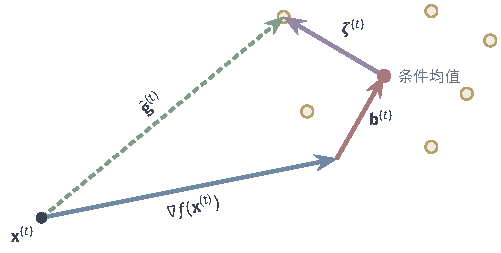
\includegraphics[width=80mm]{figures/05-optimization/05-stochastic-optimization/tikz/sgd-read-decomposition/figure.pdf}
  \caption{读数的三段分解。蓝色是真梯度，红色是条件偏差，紫色是一次读数偏离条件均值的噪声，绿色虚线是最终拿到的读数。黄色小圆是其他可能的读数，它们围绕条件均值分布。条件无偏的含义是红色线段长度为零，黄色小圆的中心落在蓝色箭头的端点上。}
  \label{fig:sgd-read-decomposition}
\end{BookInlineFigure}

图~\ref{fig:sgd-read-decomposition}说明了两部分误差的不同性质。偏差是系统性的，反复平均也去不掉；噪声的均值为零，累积时会相互抵消一部分。在二阶量上这个区别体现为交叉项消失。噪声的条件均值为零，再由规则~\eqref{eq:sgd-pull-out}，交叉项为零，于是
\begin{equation}
 \mathbb{E}[\lVert\hat{\bm{g}}^{(t)}\rVert_2^2\mid\mathcal{F}^{(t)}]
 =\lVert\nabla f(\bm{x}^{(t)})+\bm{b}^{(t)}\rVert_2^2+\mathbb{E}[\lVert\bm{\zeta}^{(t)}\rVert_2^2\mid\mathcal{F}^{(t)}].
 \label{eq:sgd-second-moment}
\end{equation}
后面的分析分别记录这两个量，噪声的条件二阶矩也称条件方差。

\paragraph{例中的偏差与方差}
三项目标上均匀抽样的读数无偏，$\bm{b}^{(t)}=0$。令$\delta=x-1$，式~\eqref{eq:sgd-example-gradients}的三个读数写成$\delta+4$，$2\delta+2$，$3\delta-6$。它们平方的平均是
\[
 \frac13\bigl[(\delta+4)^2+(2\delta+2)^2+(3\delta-6)^2\bigr]=\frac{14\delta^2-20\delta+56}{3}.
\]
减去$f'(x)^2=4\delta^2$，得到条件方差
\begin{equation}
 \sigma^2(x)=\frac{2\delta^2-20\delta+56}{3},\qquad \delta=x-1.
 \label{eq:sgd-example-variance}
\end{equation}
在$x=x^\star$处它等于$56/3\approx18.67$，这时完整梯度已经是零，噪声却最明显。在$x=2$处，$\delta=1$，方差是$38/3\approx12.67$。

式~\eqref{eq:sgd-example-variance}还说明，方差随$\lvert x\rvert\to\infty$按$\delta^2$增长。“条件方差处处不超过某个常数”这种常用假设，即使对最简单的二次目标也只在有界区域内成立。下文使用这类假设时，都理解为沿迭代点成立，它通常需要迭代点停留在有界区域内，这件事本身需要验证。

有偏的读数也容易构造。若按概率$(1/2,1/4,1/4)$抽项，又直接使用读数而不作修正，$x=2$处的条件均值是
\[
 \frac12\cdot5+\frac14\cdot4+\frac14\cdot(-3)=2.75,
\]
相对$f'(2)=2$的偏差是$0.75$。第~\ref{sec:sgd-importance}小节将说明这种偏差怎样改变实际求解的目标，以及如何用权重把它去掉。

\paragraph{无偏不保证单步下降}
条件无偏是平均意义上的性质，一次读数可能与真梯度成钝角。$x=2$处抽到第三项时，读数$-3$和真梯度$2$的乘积是$-6$，沿负读数走一步函数值上升。对比之下，条件无偏只保证
\[
 \mathbb{E}[\langle\nabla f(\bm{x}^{(t)}),\hat{\bm{g}}^{(t)}\rangle\mid\mathcal{F}^{(t)}]=\lVert\nabla f(\bm{x}^{(t)})\rVert_2^2\geq0.
\]
所以随机梯度方法不能用“每步函数值都下降”来分析，要用的是期望意义上的进展。

\subsection{循环读取与随机重排}
\label{sec:sgd-reading-orders}

上面的条件无偏依赖每步独立抽样。可在有限和目标上，常见的读取方式并不独立。

\paragraph{三种读取顺序}
有放回抽样每步独立地均匀抽一个下标，这一轮里有的项可能抽到多次，有的项可能一次也没抽到。固定循环按$1,2,\ldots,N$的顺序反复读取。\term{随机重排}（random reshuffling）每轮开始时把$N$项随机打乱一次，然后无放回地读完。把连续读取$N$项称为一\emph{轮}，后两种方式的每一轮都恰好读全部的项，图~\ref{fig:sgd-reading-orders}对比了三种方式。

\begin{BookInlineFigure}
  \centering
  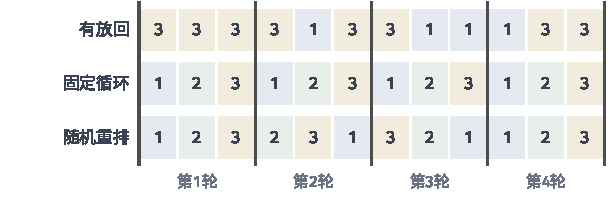
\includegraphics[width=104mm]{figures/05-optimization/05-stochastic-optimization/matplotlib/sgd-reading-orders/figure.pdf}
  \caption{三项目标在四轮内的读取顺序（种子固定）。每格的数字和底色表示读到的项，粗竖线分隔各轮。有放回抽样的一轮可能缺项、重项，固定循环每轮相同，随机重排每轮恰好各读一次，但顺序每轮不同。}
  \label{fig:sgd-reading-orders}
\end{BookInlineFigure}

\paragraph{一轮之内读数有偏}
随机重排打破了逐步条件无偏。在$x=2$处，设本轮首先读了第三项。给定这段历史，剩下两项的读数是第一项和第二项，平均后是
\[
 \frac{f_1'(2)+f_2'(2)}{2}=\frac{5+4}{2}=4.5.
\]
而完整梯度是$2$。这个偏差很好理解：读了负的一项，剩下的项一定偏正。所以式~\eqref{eq:sgd-unbiased}对随机重排的一轮内部不成立，无法直接沿用逐步的条件期望递推。

\paragraph{按整轮来分析}
偏差并不是坏事，因为一轮的总和是精确的。把一轮的$N$项读取顺序记为$\pi_0,\ldots,\pi_{N-1}$，轮内迭代点记为$\bm{x}_0,\ldots,\bm{x}_N$，步长固定为$\alpha$。把每一步的读数在轮初的点$\bm{x}_0$处展开，
\[
 \bm{x}_N=\bm{x}_0-\alpha\sum_{k=0}^{N-1}\nabla f_{\pi_k}(\bm{x}_k).
\]
一轮恰好读全部的项，所以各项读数在同一点$\bm{x}_0$处的和就是$N$倍的完整梯度。在每一项里加减$\nabla f_{\pi_k}(\bm{x}_0)$，得到
\begin{equation}
 \bm{x}_N=\bm{x}_0-\alpha N\nabla f(\bm{x}_0)-\alpha\sum_{k=0}^{N-1}\bigl[\nabla f_{\pi_k}(\bm{x}_k)-\nabla f_{\pi_k}(\bm{x}_0)\bigr].
 \label{eq:sgd-epoch-expansion}
\end{equation}
第一部分恰是步长$\alpha N$的一次完整梯度下降，与顺序无关。若各项梯度$L_i$-Lipschitz，第二部分的每一项不超过$L_i\lVert\bm{x}_k-\bm{x}_0\rVert_2$，而$\lVert\bm{x}_k-\bm{x}_0\rVert_2$本身是$\alpha$的量级，所以这部分是$\alpha^2$的量级。

一轮之内读到的梯度并不消失，它们的噪声在一轮结束时几乎抵消。有放回抽样没有这个结构，每步噪声$\alpha\bm{\zeta}^{(t)}$是$\alpha$的量级，一轮的总噪声还是$\alpha$的量级。

三项目标可以直接核对。从$x_0=2$开始，步长$\alpha=0.1$，顺序为$3,1,2$，轮内的点依次是$2.3,\ 1.77,\ 1.416$。式~\eqref{eq:sgd-epoch-expansion}的第一部分给出
\[
 2-0.1\cdot3\cdot2=1.4.
\]
第二部分的三项里，第三项在$x_0$处读取，差为零；第一项在$2.3$处读取，差是$1\cdot0.3$；第二项在$1.77$处读取，差是$2\cdot(-0.23)$。所以第二部分是
\[
 -0.1\cdot(0+0.3-0.46)=0.016,
\]
两部分合计$1.416$，与逐步计算一致。

\begin{BookInlineFigure}
  \centering
  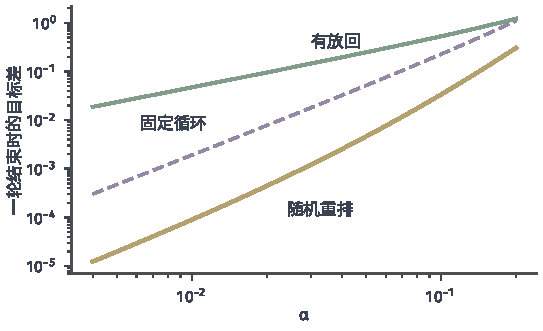
\includegraphics[width=92mm]{figures/05-optimization/05-stochastic-optimization/matplotlib/sgd-epoch-floor/figure.pdf}
  \caption{三项目标上固定步长运行至稳定后，一轮结束时的期望目标差与步长的关系，两轴都取对数。数值由精确递推算出，并非抽样估计。绿线是有放回抽样，紫色虚线是固定顺序$1,2,3$，黄线是随机重排。}
  \label{fig:sgd-epoch-floor}
\end{BookInlineFigure}

图~\ref{fig:sgd-epoch-floor}比较了固定步长长期运行后的误差。图中的三条直线斜率不同：步长缩小十倍时，有放回抽样的目标差约缩小十倍；固定循环约缩小一百倍；随机重排缩小的倍数更大，在$\alpha=0.1$和$0.01$之间约为三百七十倍，曲线向千倍的斜率靠近。在$\alpha=0.01$时，三者的目标差依次约为$4.7\times10^{-2}$，$1.9\times10^{-3}$，$9.0\times10^{-5}$。

固定循环的误差是一个确定的偏移，步长固定后迭代点按周期收敛到一条轨道，其离$x^\star$的距离是$\alpha$的量级，目标差是$\alpha^2$的量级，而且偏移大小与读取顺序有关。随机重排把各种顺序平均，轮末偏移的主要部分相互抵消。

这张图只来自一个二次例子，斜率不能直接当作一般定理。一般目标上，随机重排的结论需要对一轮的累积偏差单独分析，证明较长，读者可查阅相关文献。本章后面的逐步分析都针对有放回抽样或新样本的情形，把它们用于随机重排时要注意上面的差别。
